\chapter{Implementation, integration and test plan}

\section{Development process and approach}

The system will be implemented, integrated, and tested following a bottom-up approach, starting from the model layer and progressively adding and testing the other components of the server architecture.
This approach allows for the early validation of low-level functionalities, ensuring a solid foundation for higher-level components.

Both server-side and client-side components will be developed and tested simultaneously, but the focus will be on server-side components initially, due to their backbone role of the system.
Incremental integration testing will be applied, aiming to identify and resolve bugs as soon as they emerge during the development process, minimizing the impact on subsequent stages.

To facilitate testing at different levels of the architecture, drivers will be employed to simulate higher-level components that are not yet implemented, while stubs will be used to mock the behavior of lower-level dependencies, such as external services or the database.
This strategy ensures that individual components can be tested in isolation, while also validating their integration as part of the broader system.

This testing approach ensures that dependencies between components are carefully managed, leading to a robust and well-tested system at every level.

\section{Implementation and integeration plan}

This section describes the implementation and integration plan of each part of the system.

\subsection{Application server}

Firstly, the model and the query service will be implemented and unit tested with a driver, which will substitute components not yet implemented.

\begin{figure}[H]
    \centering
    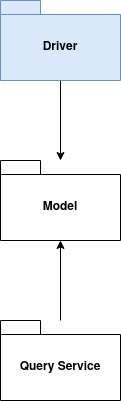
\includegraphics[width=0.1\linewidth]{../assets/implementation-plan-diagrams/implementation-plan-1.png}
\end{figure}

As the second step, the authentication service, profile manager, recommendation service, enrollment manager and internship manager will be implemented and tested with a driver, which will substitute the request dispatcher.

There will also be 3 stubs, which will substitute, respectively, the email service for the authentication service, the suggestion service for the profile manager, and the complaint manager and feedback manager for the internship manager.

\begin{figure}[H]
    \centering
    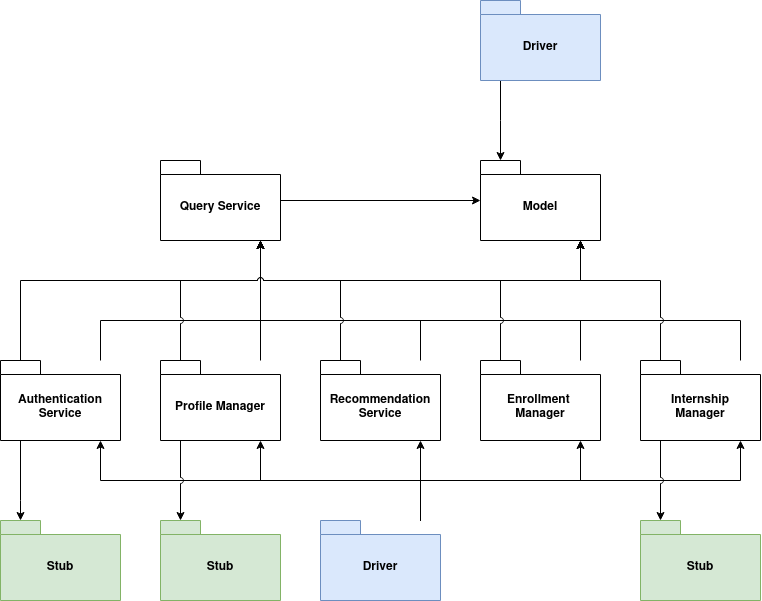
\includegraphics[width=0.7\linewidth]{../assets/implementation-plan-diagrams/implementation-plan-2.png}
\end{figure}

Then, the request dispatcher will be implemented and tested with a driver substituting the web server.

\begin{figure}[H]
    \centering
    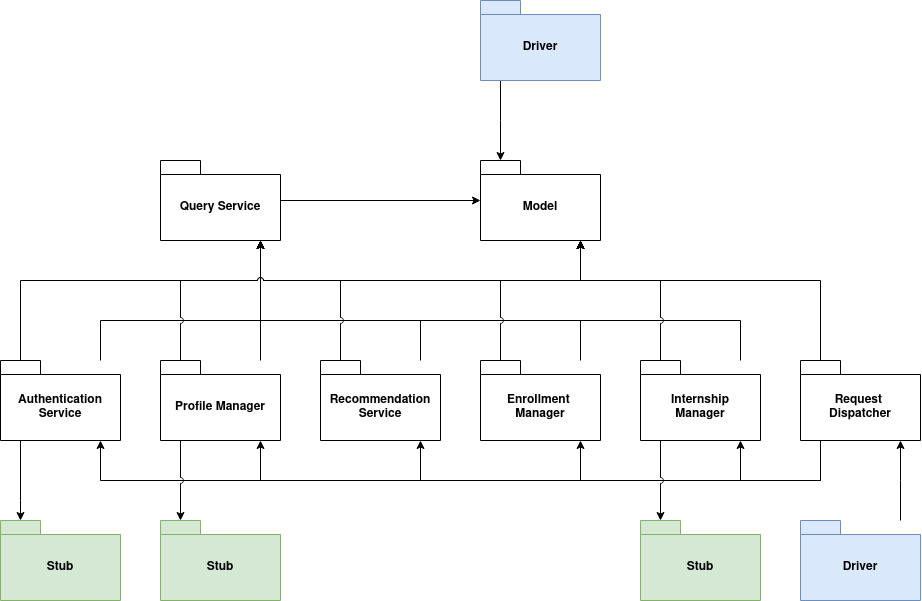
\includegraphics[width=0.8\linewidth]{../assets/implementation-plan-diagrams/implementation-plan-3.png}
\end{figure}

the last components of the server that will be implemented will be the email service, the suggestion service, the complaint manager and the feedback manager.
A stub will be used to simulate the behavior of the email server.

\begin{figure}[H]
    \centering
    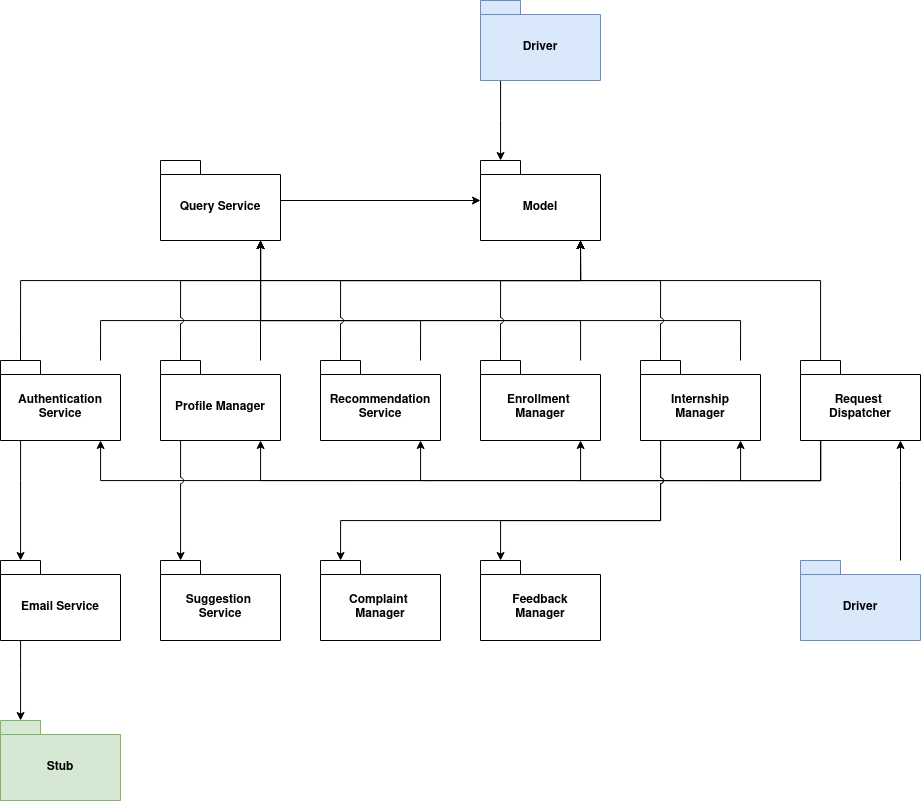
\includegraphics[width=0.8\linewidth]{../assets/implementation-plan-diagrams/implementation-plan-4.png}
\end{figure}

\subsection{Web server}

Each component of the view is rigorously unit tested using a stub for the REST APIs, enabling parallel development of the frontend and backend.

\begin{figure}[H]
    \centering
    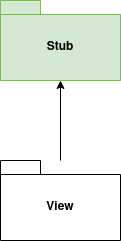
\includegraphics[width=0.1\linewidth]{../assets/implementation-plan-diagrams/implementation-plan-5.png}
\end{figure}

\subsection{Final test}

Once the implementations of the backend and of the frontend are finished, final tests can take place.

\begin{figure}[H]
    \centering
    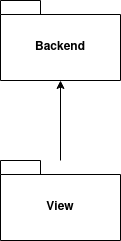
\includegraphics[width=0.1\linewidth]{../assets/implementation-plan-diagrams/implementation-plan-6.png}
\end{figure}

\section{Development technologies}

The selection of technologies for our project was the result of a careful analysis, with the goal of ensuring a system that is performant, scalable, and easily maintainable.
In this section, we will describe in detail the choices made for the web and application servers and database, highlighting the reasons behind each decision.

\subsection{Web server}

The frontend, hosted on the web server, is built using JavaScript and the React framework, along with Vite and Tailwind.
This approach allows to create responsive and easily maintainable user interfaces.
React, combined with Vite and Tailwind, offers the possibility of developing complex and dynamic
user interfaces, with excellent component management and a high-level user experience.

\subsection{Application server}

The backend of the system, deployed on the application server, is developed in C\#, with the support of the .NET runtime.
This allows to build a solid, scalable, and reliable system.
The choice of C\# and .NET was guided by their robustness, high performance, and the vast range of tools and libraries available for the development of web applications and services.

For the development of the RESTful APIs, we use the ASP.NET web framework.
This technology allows to create high-performance, efficient web services that comply with industry standards.
ASP.NET provides a flexible development environment, with a high level of performance and the ability to create well-documented APIs, which are essential for the interaction between servers.

\subsection{Database}

Data persistence is entrusted to MySQL.
This choice provides a robust database management system that is well-suited to our needs.
MySQL is a reliable and widely supported DBMS, ideal for managing relational data and its capacity to handle complex queries and large volumes of data.

The responses to database queries are provided by our MySQL system, hosted on a dedicated AWS machine.
Initially, the DBMS holds a single DB used for tests, but the architecture theoretically includes a dedicated database for production when system is ready.
The MySQL database provides a stable environment for data storage, while the logical separation between test and production ensures data integrity during development.

\subsection{Architectures and patterns}

Our system is developed following the distributed MVC pattern, with the model, view and controller components distributed between the web server, application server, and database.
We also adopt the clean architecture pattern, dividing the code into application, domain, infrastructure, and presentation modules.
The first three are found in the application server, whereas the last is on the web server.
The adoption of these patterns allows to keep the code organized, modular, and easily maintainable, promoting a clear separation of responsibilities and greater flexibility in development.

\section{Technologies used for testing}

To ensure the quality and reliability of our system, we have implemented a complete testing strategy using various tools and technologies.
In this section, we describe the choices made for unit and integration tests, as well as tools for API testing and response simulation.

\subsection{Backend unit testing}

For unit testing of the backend, we use xUnit.
This framework allows to test the components of the application server in an isolated and precise manner.
xUnit provides a flexible and complete testing environment, ideal for testing the various functionalities and logic of our system.

\subsection{Frontend unit testing}

For testing the JavaScript code of the frontend, we rely on Jest.
This framework is essential to verify the correct implementation of the user interface.
Jest provides an effective and complete testing environment for JavaScript code, allowing us to test each individual component of the frontend in isolation.

\subsection{REST APIs requests fabrication}

For creating REST requests, we use cURL and Swagger.
These tools allow to simulate and test requests efficiently.
cURL is a versatile tool for testing from the command line, while Swagger offers a graphical interface for documenting and testing APIs.

\subsection{REST APIs responses simulation}

To simulate REST responses during the frontend development, we use MSW (Mock Service Worker).
This tool allows to work independently from the backend.
MSW allows to create mock APIs without having to depend on a functioning backend, speeding up the frontend development and testing process.

\subsection{Web pages requests fabrication}

For creating web page requests, we use a web browser.
This allows to verify the interaction with the user interface.
The direct use of the browser ensures a real user experience and allows to test the functionalities of the web interface.

